\chapter{Introdução}
\label{cap-introducao}

\section{Contexto}
\label{section:contexto}

Em uma entrevista para o site da Revista Times\footciteref{Phillips2014} a Empreendedora brasileira Bel Pesce relata que em apenas duas semanas após o lançamento do seu primeiro livro na internet ele obteve mais de cem mil downloads, o que a motivou a abrir a escola de empreendedorismo FazInova\footciteref{fazinova} que no primeiro ano obteve cerca de nove mil estudantes. Hoje a plataforma possui mais de 150 mil usuários e o conteúdo criado pela Empreendedora já atingiu mais de 5 milhões de pessoas nos últimos 3 anos por meio de revistas, programas de televisão ou rádio, palestras, YouTube, etc. Ela relata que as pessoas nem sequer piscam durante as atividades e que os brasileiros querem empreender.

\citeonline{indiceglobaldoempreendedorismo} relatam que menos de 1\% das empresas do Brasil conseguem crescer mais do que 20\% ao ano por três anos consecutivos mas elas foram responsáveis por mais de 40\% dos novos empregos gerados no país, em média geram cerca de 100x mais empregos do que a média das empresas no Brasil. 

Além desse fator, \citeonline{Brinded2015} relata que o Brasil é o terceiro país com o maior número de Empreendedores do mundo, correspondendo a cerca de 13,8\% da população, o que, além de surpreendente, demonstra ser uma pauta de grande importância no Brasil. A autora explica que em países desenvolvidos os Empreendedores estão mais associados com Startups, enquanto em países menos favorecidos Empreender é mais uma questão de necessidade do que de escolha ou sonho, ela relata que as pessoas precisam criar suas próprias oportunidades quando não há muitos empregos disponíveis, por esse motivo todos os dez países com o maior número de Empreendedores do mundo são classificados como subdesenvolvidos ou em desenvolvimento, como indicado pela Tabela \ref{table:ranking_de_paises_com_mais_empreendedores}.

\begin{table}[!htb]
	\centering
	\begin{tabular}{ | p{3cm} | p{8cm} | p{4cm} | }
		\hline
		Posição & País & \% da população empreendendo \\ \hline
		1 & Uganda & 28.1 \\ \hline
		2 & Tailândia & 16.7 \\ \hline
		3 & Brasil & 13.8 \\ \hline
		4 & Camarões & 13.7 \\ \hline
		5 & Vietnam & 13.3 \\ \hline
		6 & Angola & 12.4 \\ \hline
		7 & Jamaica & 11.9 \\ \hline
		8 & Botsuana & 11.1 \\ \hline
		9 & Chile & 11.0 \\ \hline
		37 & Reino Unido & 4.6 \\ \hline
		41 & Estados Unidos da América & 4.3 \\ \hline
	\end{tabular}
	\caption{Ranking de países com a maior proporção de Empreendedores, por \cite{Brinded2015}}	\label{table:ranking_de_paises_com_mais_empreendedores}
\end{table}

\citeonline{Hermann2015} no Índice Global de Ecossistemas de Startups classifica uma cidade brasileira, São Paulo, como o 12o melhor Ecossistema do mundo, a frente de cidades como Austin, Toronto, Amsterdã e Montreal. \citeonline{schwab2015} já não classifica tão bem o Brasil, no Índice Global de Competitividade fomos classificados na 75a posição dentre 140 países. No Índice Global de Empreendedorismo, criado por \citeonline{Acs2016}, somos classificados na posição 92 do ranking global, um dos destaques do Brasil segundo esse Índice está no pilar de Percepção de Oportunidade que estamos posicionados em primeiro lugar, como indicado pela Figura \ref{figure:gedi_brazil}.

\begin{figure}[!htb]
	\centering
	\includegraphics[width=11cm,angle=0]{figuras/gedi_brazil}
	\caption{Comparação dos pilares brasileiros de acordo com o Índice Global de Empreendedorismo}
	\label{figure:gedi_brazil}
\end{figure}

O Governo também tem dado apoio a esse setor por meio de iniciativas como o Startup Brasil, Inovativa Brasil, Sebrae de Inovacão, Editais de investimento como os da FINEP, dentre outros. Alguns projetos de lei como a Lei da Inovação e o Marco Legal da Ciência, Tecnologia e Inovação busca flexibilidade o atual Ambiente Regulatório do Brasil para aumentar as chances de sucesso das Startups. 

Alguns Grupos não-governamentais como o Dínamo promovem discussões sobre Startups com foco na criação de políticas públicas mais favoráveis no Brasil, parte do trabalho deles também visa apoiar Governos na formulação dessas políticas e aproxima-los do Ecossistema. A ANPROTEC relata que empresas apoiadas por incubadoras no Brasil faturam em torno de R\$ 15 bilhões anuais e são responsáveis por cerca de 53 mil empregos para o Brasil. Eles estimam que existam cerca de 369 incubadoras de empresas e cerca de 5000 empresas associadas a elas, sejam já graduadas ou ainda em fase de incubação\footciteref{Anprotec2016}, e podem ser vistas como Startups. 

\citeonline{Paternoster2014} enfatiza que pesquisas acadêmicas são necessárias para apoiar as atividades relacionadas a Startups e guiar ações de diversos atores que compõem um Ecossistema, como Empreendedores, Agentes Públicos, Investidores e Acadêmicos. \citeonline{Filion1998} relata que estudos relacionados ao Empreendedorismo são antigos, alguns datando meados do século XIX, e embora ainda não haja um consenso sobre qual a sua definição sabemos que é uma disciplina que pode ser aprendida, as pessoas não nascem Empreendedoras mas são criadas e treinadas para se tornarem Empreendedoras. Com base em uma análise das principais publicações acerca do tema nos últimos 300 anos o autor divide o progresso dos estudos em cinco períodos representados pela Tabela \ref{table:tendencias_nas_publicacoes_acerca_do_empreendedorismo}. Filion também mapeou quais os principais tópicos de pesquisa, o resultado está na Tabela \ref{table:principais_temas_de_pesquisa_na_area_de_empreendedorismo}.

\begin{table}[!htb]
	\centering
	\begin{tabular}{ | p{6cm} | p{6cm} | p{3cm} | }
		\hline
		Tema & Perspectiva & Período \\ \hline
		O que fazem os Empreendedores & Econômica & 1700 - 1950 \\ \hline
		Quem são os Empreendedores & Comportamental & 1960 - 1980 \\ \hline
		O que fazem os Empreendedores & Administrativa(finanças, marketing, operações, recursos humanos) & 1980 - Atual \\ \hline
		Quais tipos de suporte são necessários para Empreendedores & Ciências Sociais(incluindo economia, geográfia e sociologia) & 1985 - Atual \\ \hline
		O que são atividades Empreendedoras e quais Competências são necessárias & Empreendedorismo & 1990 - Atual \\ \hline
	\end{tabular}
	\caption{Tendências nas publicações acerca do Empreendedorismo por \cite{Filion1998}}	
	\label{table:tendencias_nas_publicacoes_acerca_do_empreendedorismo}
\end{table}

\begin{table}[!htb]
	\centering
	\begin{tabular}{ | p{15cm} |}
		\hline
		Temas de Pesquisa \\ \hline
		Características comportamentais de Empreendedores \\ \hline
		Características demográficas e econômicas de pequenos negócios \\ \hline
		Empreendedorismo e pequenos negócios em países em desenvolvimento \\ \hline
		Características gerenciais de Empreendedores \\ \hline
		Criação de empresas \\ \hline
		Desenvolvimento de negócios \\ \hline
		Capital de risco e investimento em pequenos negócios \\ \hline
		Gestão de negócios, recuperação e aquisição \\ \hline
		Estratégia e crescimento de uma companhia empreendedora \\ \hline
		Alianças estratégicas \\ \hline
		Empreendedorismo corporativo e intraempreendedorismo \\ \hline
		Negócios de família \\ \hline
		Encubadoras e sistemas de suporte ao Empreendedorismo \\ \hline
		Redes \\ \hline
		Fatores que influenciam a criação e o desenvolvimento de empresas \\ \hline
		Políticas públicas governamentais e criação de empresas \\ \hline
		Mulheres, minorias, grupos étnicos e Empreendedorismo \\ \hline
		Educação Empreendedora \\ \hline
		Pesquisa Empreendedora \\ \hline
		Comparativo de estudos culturais\\ \hline
		Empreendedorismo e a Sociedade \\ \hline
		Franquias \\ \hline
	\end{tabular}
	\caption{Principais temas de pesquisa na área de Empreendedorismo por \cite{Filion1998}}
	\label{table:principais_temas_de_pesquisa_na_area_de_empreendedorismo}
\end{table}

Como explicitado por \citeonline{Filion1998} em 1998, pouco se explorou sobre Ecossistemas e como eles contribuem para o desenvolvimento da economia, das empresas e das pessoas que os cercam, embora seja claro que algo de diferente aconteça em grandes Ecossistemas como o Vale do Silício, Nova Iorque ou Tel-Aviv. Alguns pesquisadores, como \citeonline{Suresh2012}, tentaram mapear elementos que são essenciais e como interagem entre si para que um determinado Ecossistema possa crescer.

Contextualizando com anos mais recentes, \citeonline{Cukier2016} mapeou o crescimento da quantidade de artigos acadêmicos que citam o termo ``Startup Ecosystems'', como representado na Figura \ref{figure:papers_about_startup_ecosystems}, mostrando um considerável aumento no interesse pelo tema. \citeonline{Lemos2011} diz que pesquisas sobre Ecossistemas de Empreendedorismo apresentam um forte caráter exploratório e que faltam teorias consolidadas sobre as relações entre os diversos elementos que compõem um Ecossistema. \citeonline{Spigel2015} também relata que o estudo de Ecossistemas Empreendedores se tornaram uma ferramenta popular para o estudo do empreendedorismo de alto crescimento com um ponto de vista geográfico. Como sugerido e feito por \citeonline{Sun2011}, a ferramenta Google Ngram lista a frequência com que um determinado termo é mencionado em livros e a curva do termo ``startups'' é deveras interessante, como representado pela Figura \ref{figure:startupngram}. O termo começou a ser usado de forma constante em meados de 1960, teve um grande crescimento a partir de 1980 e uma queda a partir de 2002, pouco depois da bolha pontocom. Infelizmente a plataforma ainda não possui dados após 2008, quando o uso do termo pareceu voltar a crescer. 

\begin{figure}[!htb]
	\centering
	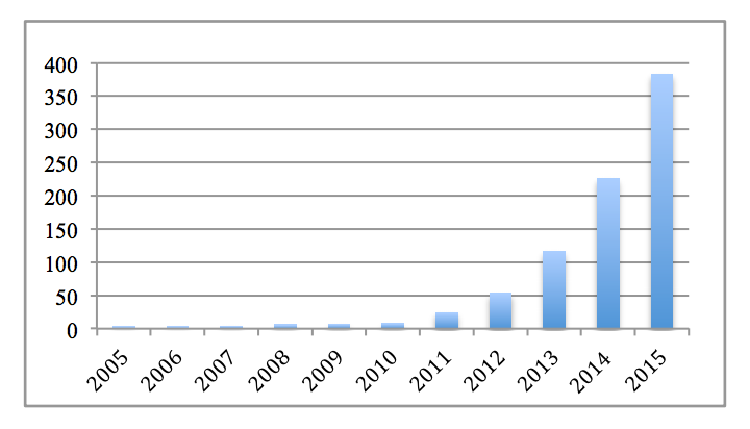
\includegraphics[width=11cm,angle=0]{figuras/papers_about_startup_ecosystems}
	\caption{Quantidade de Papers com o termo ``Startup Ecosystem'' por \citeonline{Cukier2016}}
	\label{figure:papers_about_startup_ecosystems}
\end{figure}

\begin{figure}[!htb]
	\centering
	\includegraphics[width=11cm,angle=0]{figuras/startupngram}
	\caption{Referência ao termo ``startups'' de acordo com o Google Ngram}
	\label{figure:startupngram}
\end{figure}

Trazendo para o contexto de Brasília, a cidade vive um dos seus melhores momentos para o crescimento do Ecossistema de Startups local, embora o país e a cidade estejam passando por uma recessão e crise política e econômica o cenário nunca foi tão favorável e como reflexo é vísivel que o interesse dos brasilienses tem aumentado. \citeonline{Sun2011} relata que a Professora da Harvard Business School Janet. J. Kraus acredita que as crises são os melhores momentos para se iniciar um novo negócio, justamente quando os custos de oportunidade são baixos. Ela defende que se o Empreendedor é capaz de lucrar durante uma crise então o negócio será ainda mais lucrativo quando o mercado se recuperar.

Atualmente é possível encontrar eventos com temáticas relacionadas ao Empreendedorismo, como palestras e meetups, no mínimo uma vez por semana. A expectativa para 2016 e 2017 também é boa: grandes eventos como a WCIT, que estima-se que poderá gerar bilhões de reais em negócios entre um público seleto de 2500 participantes, em sua maior parte líderes das principais empresas do setor, o Festival Path e a Campus Party também acontecerão em Brasília. 

A baixa expectativa de concursos públicos também é um fator favorável, forçando os jovens a buscarem alternativas que não a estabilidade financeira incentivada pelos seus pais, principal motivo para uma Cultura Empreendedora tão ruim na cidade. 

Em relação a financiamento existem dois fundos de alto risco com aproximadamente R\$ 100 milhões para investimento em Startups, o Criatec 2, sob resposabilidade da Garan Ventures, e o Fundo de Investimento em Participações Venture Brasil Central, sob responsabilidade da Cedro Capital. Também temos três programas de aceleração de Startups rodando na cidade, o Programa Impulso, o CAMP da aceleradora Cotidiano, e a Acceleratus. A presença de cerca de dez espaços de coworking e duas incubadoras também atuam como importantes atores para o desenvolvimento do Ecossistema.

O Governo de Brasília também busca por meios de apoiar o Ecossistema local, a Fundação de Apoio à Pesquisa em 2015 e 2016 investiu cerca de R\$ 13 milhões em Startups locais. A Secretaria de Ciência, Tecnologia e Inovação além de coordenar o Parque Tecnológico Capital Digital, uma área com mais de 1 milhão de metros quadrados exclusiva para negócios relacionados à Tecnologia da Informação, está desenvolvendo um anteprojeto de lei da inovação o qual propõem isenção total de impostos para Startups por até 4 anos. 

De acordo com \citeonline{indiceglobaldoempreendedorismo} em 2016 Brasília obteve ótimos indicadores de Mercado e Acesso à Capital, mas não se destacou em Ambiente Regulatório, Inovação, Capital Humano e demonstrou resultados muito ruins em Infraestrutura e Cultura Empreendedora. Os resultados e a comparação com Goiânia estão representados na Figura \ref{figure:indice_de_cidades_empreendedoras_brasilia_e_goiania}.

\begin{figure}[!htb] 
\centering
\includegraphics[width=11cm,angle=0]{figuras/indice_de_cidades_empreendedoras_brasilia_e_goiania}
\caption{Análise de Brasília no Índice de Cidades Empreendedoras, da Endeavor}
\label{figure:indice_de_cidades_empreendedoras_brasilia_e_goiania}
\end{figure}

A capital também é a casa de diversos casos de sucesso no contexto de Startups do Brasil. Em entrevista ao Correio Braziliense\footciteref{menezes2012} Júlio Vasconcellos, ex-morador de Brasília e um dos fundadores do Peixe Urbano, acredita que a capital possui um excelente sistema de educação e jovens com talento e ambição e que o contexto político da cidade, que atrai muitos estrangeiros e brasileiros de todas as regiões do país, contribui para a geração de um ambiente dinâmico e favorável para o desenvolvimento de jovens empreendedores. A Boo-Box, uma das maiores empresas de publicidade digital do mundo e adquirida pela FTPI Digital, a ZeroPaper, adquirida pela americana Intuit, a Rota dos Concursos, a primeira Startup brasileira a participar do programa de aceleração 500 Startups no Vale do Silício, também são grandes nomes da capital. Em 2016, a Tradr, criada em Brasília, recebeu o prêmio de melhor Startup na área de e-commerce na Campus Party Brasil.

\section{Objetivos}
\label{section:objetivos}

O objetivo deste trabalho consiste em um estudo de caráter exploratório do Ecossistema de Startups de Brasília com o objetivo de conhece-lo com o objetivo de avaliar seu atual momento e sua maturidade. Como resultado final é esperado um Mapa Conceitual, uma síntese dos dados coletados de forma a permitir comparações com outros Ecossistemas globais que foram avaliados com a mesma metodologia e uma visão generalista de algumas das características do Ecossistema de acordo com as visões dos Empreendedores locais, bem como algumas sugestões de ações que poderiam ser tomadas de forma a sanar alguns dos problemas identificados no Ecossistema.

\section{Organização do Trabalho}
\label{section:organizacao_do_trabalho}

Este trabalho está organizado em cinco capítulos: o primeiro, este, com uma breve introdução de suas motivações, objetivos e contexto. 

O segundo capítulo, com foco na Fundamentação Teórica trás diversos conceitos e visões relativos ao Empreendedorismo, sobre quem é o Empreendedor e o que é uma Startup, bem como o seu Ciclo de Vida e o seu mercado fora do convencional. 

O terceiro capítulo explora a Metodologia utilizada, como as entrevistas foram realizadas, como esse trabalho se relaciona com outros similares, etc. 

O quarto capítulo trás os Resultados Obtidos, o que foi descoberto, qual a visão dos Empreendedores entrevistados, etc.

No último capítulo, o de Conclusões, é feito um apanhado de tudo o que foi explorado nos capítulos anteriores e o que fora aprendido sobre o Ecossistema de Startups do Distrito Federal e quais ações poderiam ser tomadas para que Brasília se torne uma cidade mais empreendedora.